\section{Results}
To record results we computed the statistics using a thirty second bathymetry grid.
The grid was chosen because of the size and complexity of the computations.
This grid will give good results for potential runtimes and allow to anticipated the time scaled to larger resolutions
Included in the results is a time for a Fortran implementation.
Fortran was the original language for these grid computations.
These programs did not scale well for larger resolution grids.
We only recorded the execution times for the Java and OpenMP implementations.
This is because of the preformance issues we experienced with the MPI implementation.

\par
The Mean and Standard deviation times are shown in Figure 3.
All results were timed in hours for each coresponding core ammount.
The mean and standard deviation graph shows a obvious curve.
\begin{figure}[h]
    \centering
    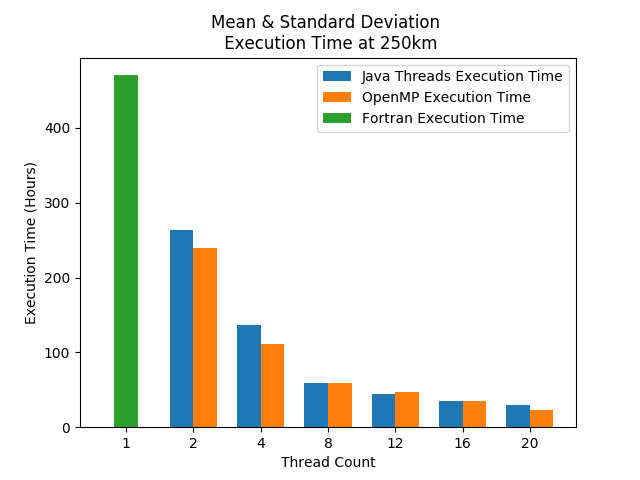
\includegraphics[scale=0.5]{merp}
    \caption{Results for Mean and Standard Deviation}
    \label{fig:3}
\end{figure}

\par
Java threads preformed marginally slower than the C implementation.
The slow down scaled well with more cores used in computation.
Going from several days to only several hours at higher core count.

\par
The Plane fit results are shown in Figure 4.
The original Fortran program required months to run.
However, we timed the Java implementation at around two weeks for 20 cores.
We did not run it at lower core counts for sake of time.
Predicting based on previous trends the time requirements will be several months.

\begin{figure}[h]
    \centering
    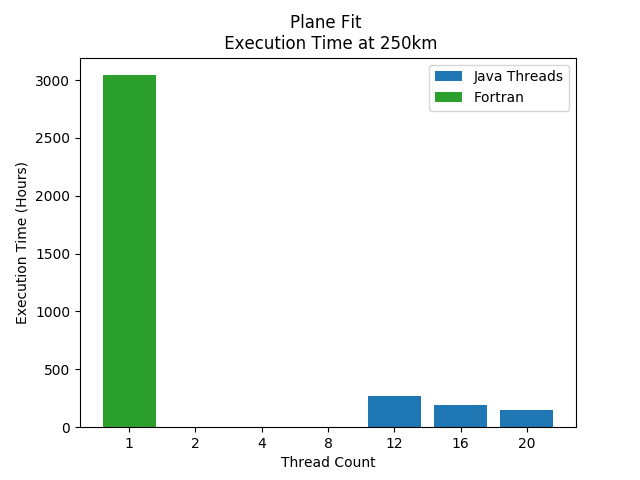
\includegraphics[scale=0.5]{plane}
    \caption{Results for Plane Fit}
    \label{fig:4}
\end{figure}

